\mode<article>{
	\clearpage
}

\section{Interfaces}

\mode<presentation>{
\begin{frame}
	\frametitle{Core TLM2 interfaces}
	\begin{block}{Definition}
		An interface is the way modules use to communicate between each
		other.
	\end{block}
	\begin{itemize}
		\item<1-> TLM2 keeps the core interfaces from TLM1.
		\item<1-> TLM2 adds the following interfaces:
		\begin{itemize}
			\item<1-> blocking and non-blocking transport interfaces,
			\item<1-> a direct memory interface (DMI), and
			\item<1-> a debug transaction interface.
		\end{itemize}
	\end{itemize}
\end{frame}
}

\mode<article>{
As we have seen for Cycle Level Modeling modules used ports to communicate with each other.
With Transaction Level Modeling modules still use ports, however they are quite different.
Ports under TLM are attached to interfaces, those are methods that are implemented by the target module.
TLM2 defines a series of interfaces that the programmer can use to implement his/her TLM simulator.

TLM2 for compatibility issues kept the interfaces defined by TLM1, so previous simulators using TLM1 interfaces could be used with the new TLM definition.
However, the TLM Accellera working group recommends to build new modules using TLM2 interfaces and writing rules.
For this reason we are not going to explain TLM1 interfaces and focus only on the new TLM2 interfaces.

In the following subsections the TLM2 interfaces will be introduced in detail:
\begin{itemize}
	\item the blocking transport interface,
	\item the non-blocking transport interface,
	\item the direct memory interface (DMI), and
	\item the debug transaction interface.
\end{itemize}
}

\subsection{Blocking transport interface}

\mode<presentation>{
\begin{frame}
	\frametitle{Blocking transport interface}
	\setbeamercolor{postit}{fg=black,bg=yellow}
	\begin{beamercolorbox}[center,rounded=true,wd=\textwidth]{postit}
		Designed for the untimed and loosely-timed coding style.
	\end{beamercolorbox}
	\begin{itemize}
		\item<1->Definition:
	\begin{figure}[h]
		\lstinputlisting{tlm/b_transport.cc}
	\end{figure}
		\item<2->The \texttt\textbf{TRANS} argument is by default set to \texttt{\textbf{tlm\_generic\_payload}}.
		\item<3->Recommended to use the generic payload for interoperability issues.
		\item<4->\texttt{sc\_time} parameter: precise simulation time (relative to the last synchronization) the call is taking place.
	\end{itemize}
\end{frame}

\begin{frame}
	\frametitle{Blocking transport interface: Rules (I)}
	\begin{enumerate}
	\item The caller is responsible for allocating storage and for constructing the transaction object. 
	The \texttt{\textbf{b\_transport}} method shall be called with a fully initialized transaction object.
	\item In the case of the generic payload, the call to \texttt{\textbf{b\_transport}} shall mark the first timing point of the transaction.
	The return from \texttt{\textbf{b\_transport}} shall mark the final timing point of the transaction.
	\item The callee may modify or update both the transaction object or the time. Modifications of the transaction object is subject to any constraints imposed by the transaction class \texttt{\textbf{TRANS}}.
	\item The caller is responsible for deleting or pooling the transaction object after the call.
	\end{enumerate}
\end{frame}

\begin{frame}
	\frametitle{Blocking transport interface: Rules (II)}
	\begin{enumerate}
	\item The callee shall assume that the caller will invalidate the transaction object upon return from \texttt{\textbf{b\_transport}}.
	\item The \texttt{\textbf{b\_transport}} method supports temporal decoupling.
	\item It is recommended that the transaction object should not contain timing information. 
	\item \texttt{\textbf{b\_transport}} may make one or several calls to \texttt{\textbf{nb\_transport\_fw}}. 
	It is straightforward to create an adapter between an untimed or loosely-timed initiator and an approximately-timed target.
	\end{enumerate}
\end{frame}
}

\mode<article>{
The TLM2 blocking interface supports an untimed and loosely-timed modeling style.
It defines the \texttt{\textbf{b\_transport}} method, which takes two non-const reference arguments, used by the source module to set the message and emission time and by the target module to set the response and update time. 
Figure~\ref{fig:b_transport_definition} shows the blocking interface definition.
\begin{figure}[h]
	\lstinputlisting{tlm/b_transport.cc}
	\caption{The blocking transport interface class definition.}
	\label{fig:b_transport_definition}
\end{figure}

\subsubsection{The \texttt{TRANS} template argument}
The purpose of this interface (and of the non-blocking interfaces that we will see later) is to make possible transport transactions of any type.
However, for a maximum interoperability between modules of different constructors a default transaction type is proposed: the \texttt{\textbf{tlm\_generic\_payload}}.

Applications should use the default transaction type \texttt{\textbf{tlm\_generic\_payload}} or extend it if needed. 
We will see the specifics of the generic payload and how it can be extended later in this chapter.

The initiator is responsible for the allocation of the transaction object and its destruction once the response has been received.
The target module can only use the received transaction object during the call of the \texttt{\textbf{b\_transport}}, after that it must suppose that the transaction object no longer exists.

\subsubsection{Rules}
When using the blocking transport interface the following rules must be followed:
\begin{enumerate}
	\item The caller is responsible for allocating storage and for constructing the transaction object. 
	The \texttt{\textbf{b\_transport}} method shall be called with a fully initialized transaction object.
	\item In the case of the generic payload, the call to \texttt{\textbf{b\_transport}} shall mark the first timing point of the transaction.
	The return from \texttt{\textbf{b\_transport}} shall mark the final timing point of the transaction.
	\item The callee may modify or update the transaction object, subject to any constraints imposed by the transaction class \texttt{\textbf{TRANS}}.
	\item The caller is responsible for deleting or pooling the transaction object after the call.
	\item The callee shall assume that the caller will invalidate the transaction object upon return from \texttt{\textbf{b\_transport}}.
	\item The \texttt{\textbf{b\_transport}} method supports temporal decoupling.
	\item It is recommended that the transaction object should not contain timing information. 
	\item \texttt{\textbf{b\_transport}} may make one or several calls to \texttt{\textbf{nb\_transport\_fw}}. 
	It is straightforward to create an adapter between an untimed or a loosely-timed initiator and an approximately-timed target.
\end{enumerate}
}

\subsection{Non-blocking transport interfaces}

\mode<presentation>{
\begin{frame}
	\frametitle{Non-blocking transport interfaces}
	\setbeamercolor{postit}{fg=black,bg=yellow}
	\begin{beamercolorbox}[center,rounded=true,wd=\textwidth]{postit}
		Designed for the approximately-timed coding style.
	\end{beamercolorbox}
	\begin{figure}[h]
		\lstinputlisting{tlm/nb_transport.cc}
	\end{figure}
\end{frame}

\begin{frame}
	\frametitle{Non-blocking transport interfaces (II)}
	\begin{itemize}
		\item Must be defined by both initiator and target.
		\begin{center}
			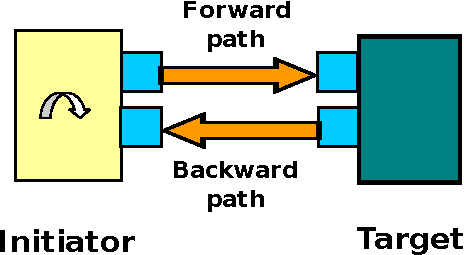
\includegraphics[width=0.6\textwidth]{tlm/figures/nb_fig.pdf}
		\end{center}
		\item Parameters and return value:
		\begin{itemize}
			\item The transaction (\texttt{tlm\_generic\_payload}).
			\item \texttt{\textbf{PHASE}} indicates the state of the transaction: \texttt{\textbf{BEGIN\_REQ}}, \texttt{\textbf{END\_REQ}}, \texttt{\textbf{BEGIN\_RESP}}, and \texttt{\textbf{END\_RESP}}.
			\item The \texttt{sc\_time} parameter indicates the precise simulation time (relative to the last synchronization) the call is taking place.
			\item The return value (\texttt{tlm\_sync\_enum}) indicates the  call status, and fixes synchronization points.
		\end{itemize}
	\end{itemize}
\end{frame}

\begin{frame}
	\frametitle{Non-blocking transport interfaces: Rules (I)}
	\begin{enumerate}
		\item The \texttt{\textbf{nb\_transport\_fw}} and \texttt{\textbf{nb\_transport\_bw}} methods shall not call wait, directly or indirectly.
		\item The \texttt{\textbf{nb\_transport\_fw}} and \texttt{\textbf{nb\_transport\_bw}} methods may be called from a thread process or from a method process.
		\item With the approximately-timed coding style, \texttt{\textbf{nb\_transport\_fw}} and \texttt{\textbf{nb\_transport\_bw}} are called respectively along the forward and backward paths between initiator and target.
		In the case of the generic payload, the two paths should pass through exactly the same sequence of components and sockets, obviously in reverse order.
	\end{enumerate}
\end{frame}

\begin{frame}
	\frametitle{Non-blocking transport interfaces: Rules (II)}
	\begin{enumerate}
		\item The initiator is responsible for deleting or pooling the transaction object after the final timing point. 
		\item If an interconnect component or a target needs to access the state of the transaction after the final call to \texttt{\textbf{nb\_transport\_fw}} or \texttt{\textbf{nb\_transport\_bw}} for a particular transaction instance, it must make a copy of the transaction object.
		\item A \texttt{\textbf{nb\_transport\_fw}} call on the forward path shall under no circumstances directly or indirectly make a call to \texttt{\textbf{nb\_transport\_bw}} on the associated backward path, and vice versa.
	\end{enumerate}
\end{frame}

\begin{frame}
	\frametitle{\small Non-blocking transport interfaces: The \texttt{phase} argument}
	\vspace{0.4em}
	\setbeamercolor{postit}{fg=black,bg=yellow}
	\begin{beamercolorbox}[center,rounded=true,wd=\textwidth]{postit}
		It serves to program protocols phases.
	\end{beamercolorbox}
	\begin{itemize}
		\item<1-> Both caller and callee can modify its value.
		\item The \texttt{tlm\_phase} enum defines four different phase status:
		\begin{itemize}
			\item<1-> \texttt{BEGIN\_REQ}
			\item<1-> \texttt{END\_REQ}
			\item<1-> \texttt{BEGIN\_RESP}
			\item<1-> \texttt{END\_RESP}
		\end{itemize}
	\end{itemize}
	\onslide<2->
	\vspace{-0.9em}
	\begin{center}{
	\scriptsize
	\begin{tabular}{|l|l|l|}
		\hline
		\texttt{\textbf{tlm\_phase}} & \textbf{Coding style} & \textbf{Path} \\
		\hline
		\texttt{BEGIN\_REQ} & Loosely- and approximately-timed & Forward(call) \\
		\hline
		\texttt{END\_REQ} & Approximately-timed only & Forward(return) \\
		& & Backward(call) \\
		\hline
		\texttt{BEGIN\_RESP} & Loosely- and approximately-timed & Forward(return) \\
		& & Backward(call) \\
		\hline
		\texttt{END\_RESP} & Approximately-timed only & Forward(call) \\
		& & Backward(return) \\
		\hline
	\end{tabular}
	}
	\end{center}
\end{frame}

\begin{frame}
	\frametitle{\small Non-blocking transport interface: The \texttt{sc\_time} argument}
	\setbeamercolor{postit}{fg=black,bg=yellow}
	\begin{beamercolorbox}[center,rounded=true,wd=\textwidth]{postit}
		It is used to indicate when the current transaction phase is taking place.
	\end{beamercolorbox}
	\begin{itemize}
		\item<1-> It is always a positive number.
		\item<1-> It is relative to the current simulation time, as returned from \texttt{sc\_time\_stamp}.
	\end{itemize}
	\onslide<2->
	\begin{block}{Temporal decoupling}
		Thanks to this argument the simulators can implement \emph{temporal decoupling}, that is running without yielding control (calling \texttt{wait(\ldots)}) to the SystemC scheduler.
		\newline \newline
		\emph{This enhances the performance of the simulator.}
	\end{block}
\end{frame}

\begin{frame}
	\frametitle{\small Non-blocking transport interface: \texttt{tlm\_sync\_enum} return arg.}
	\setbeamercolor{postit}{fg=black,bg=yellow}
	\begin{beamercolorbox}[center,rounded=true,wd=\textwidth]{postit}
		It signals if the call was a success or something failed, and if a synchronization is needed.
	\end{beamercolorbox}
	Four possible values:
	{\footnotesize
	\definecolor{MyDarkGreen}{rgb}{0,0.45,0}
	\newcommand{\X}{\textbf{\color{MyDarkGreen}$\surd$}}
	\newline
	\begin{tabular}{|l|p{2.5em}|p{2.5em}|l|l|}
		\hline
		\texttt{\textbf{tlm\_sync\_enum}} & \multicolumn{2}{l|}{\textbf{Coding style}} & \textbf{Transaction and} & \textbf{Timing} \\
		\cline{2-3}
		& {\protect \centering LT} & {\protect \centering AT} & \textbf{phase arguments} & \textbf{annotation} \\
		\hline
		\texttt{TLM\_ACCEPTED} & \X & \X & Unmodified &  \\
		\hline
		\texttt{TLM\_UPDATED} & & \X & Updated & \X \\
		\hline
		\texttt{TLM\_COMPLETED} & \X & \X & Updated\tiny{(but caller} & \X \\
		& & & \tiny{may ignore phase)} & \\
		\hline
	\end{tabular}
	}
\end{frame}
}

\mode<article>{
The non-blocking transport interfaces exist to support the loosely-timed and approxitemately-timed coding styles.
Figure~\ref{fig:nb_transport_definition} shows the non-blocking transport interfaces definitions.

\begin{figure}[h]
	\lstinputlisting{tlm/nb_transport.cc}
	\caption{The non-blocking transport interfaces class definitions.}
	\label{fig:nb_transport_definition}
\end{figure}

The non-blocking transport interfaces defines the \texttt{\textbf{nb\_transport\_fw}} and \texttt{\textbf{nb\_transport\_bw}} methods which, as the blocking transport interface method \texttt{\textbf{b\_transport}}, passes a non-const reference to the transaction object.
The \texttt{\textbf{nb\_transport\_fw}} and \texttt{\textbf{nb\_transport\_bw}} methods also passe two other parameters:
\begin{itemize}
	\item a non-const reference to a \texttt{\textbf{PHASE}} object to indicate the state of the transaction, and
	\item a time to annotate the delay of the next phase transition.
\end{itemize}
Additionally the \texttt{\textbf{nb\_transport\_fw}} and \texttt{\textbf{nb\_transport\_bw}} methods can return a value (\texttt{\textbf{tlm\_sync\_enum}}) to indicate the status of the call, and signal synchronization points. 

Unlike the blocking transport interface, the non-blocking transport interfaces needs to be defined by both, the initiator and the target modules.
That is, there is a forward non-blocking transport interface used by the initiator to send requests and a backward non-blocking transport interface used by the target to send the responses.

\subsubsection{Rules}
When using the non-blocking transport interface the following rules must be followed:
\begin{enumerate}
	\item The \texttt{\textbf{nb\_transport\_fw}} and \texttt{\textbf{nb\_transport\_bw}} methods shall not call wait, directly or indirectly.
	\item The \texttt{\textbf{nb\_transport\_fw}} and \texttt{\textbf{nb\_transport\_bw}} methods may be called from a thread process or from a method process.
	\item Exceptionally, if both the blocking and non-blocking transport interfaces are being used together, \texttt{\textbf{nb\_transport\_fw}} may need to call \texttt{\textbf{b\_transport}}. 
	This is only technically possible if it can be guaranteed that the \texttt{\textbf{b\_transport}} method does not call wait, directly or indirectly, but is in any case bad practice.
	Otherwise, the solution is to call to \texttt{\textbf{b\_transport}} from a separate thread process, spawned or notified by the original \texttt{\textbf{nb\_transport\_fw}} call.
	\item With the approximately-timed coding style, \texttt{\textbf{nb\_transport\_fw}} and \texttt{\textbf{nb\_transport\_bw}} mathod are called respectively along the forward and backward paths between initiator and target. 
	In the case of the generic payload, the two paths should pass through exactly the same sequence of components and sockets, obviously in reverse order.
	\item The initiator is responsible for deleting or pooling the transaction object after the final timing point. 
	The final timing point may be marked by a call to or a return from either \texttt{\textbf{nb\_transport\_fw}} on the forward path or \texttt{\textbf{nb\_transport\_bw}} on the backward path. 
	If the final call to non-blocking transport interfaces is on the forward path (i.e. \texttt{\textbf{nb\_transport\_fw}}), the initiator may delete the transaction object on return from \texttt{\textbf{nb\_transport\_fw}}.
	If the final call to non-blocking transport interface is on the backward path (i.e. \texttt{\textbf{nb\_transport\_bw}} , the initiator may delete the transaction object the next time the initiator process resumes, in which case the transaction object shall remain valid and accessible by the target until the target yields to the SystemC scheduler. 
	In other words, if the final call to non-blocking transport interfaces is from target to initiator, the target has a chance to inspect the state of the transaction object before it yields control. 
	After that, any interconnect component or target must assume that the transaction object is invalid.
	\item If an interconnect component or a target needs to access the state of the transaction after the final call to non-blocking transport interfaces for a particular transaction instance, it must make a copy of the transaction object.
	\item A call to non-blocking transport interfaces on the forward path shall under no circumstances directly or indirectly make a call to non-blocking transport interfaces on the associated backward path, and vice versa.
\end{enumerate}

\subsubsection{The \texttt{TRANS} template argument}
The same rules that apply to the transport blocking interface are applied to the non-blocking interface.
However, it must be noted that the life of the transaction expands from the forward request from the initiator starting the request to the backward response from the target module.

\subsubsection{The \texttt{phase} argument}
The phase argument serves to program protocols phases.
The generic payload uses the specific enum \texttt{\textbf{tlm\_phase}}.
Other protocols may substitute it with their own phase types, but this will imply a loss of interoperability.

The \texttt{\textbf{phase}} argument is passed as a non-const reference, which means that both the caller and the callee can change its value.

The \texttt{\textbf{tlm\_phase}} enum defines four different phase status:
\begin{itemize}
	\item \texttt{\textbf{BEGIN\_REQ}}: it marks the beginning of the transaction request.
	It can be used by the approximately-timed coding style.
	The initiator uses this phase when starting a non-blocking transport transaction.
	\item \texttt{\textbf{END\_REQ}}: it marks the end of the transaction request.
	It is only used for the approximately-timed coding style.
	The target uses this phase when finishing a non-blocking transport transaction.
	\item \texttt{\textbf{BEGIN\_RESP}}: it is used by the callee to mark the beginning of the transaction response.
	It can be used by the approximately-timed coding style.
	The transaction callee module can start the response at different points, for example setting the forward call phase argument when returning from a \texttt{\textbf{BEGIN\_REQ}} or \texttt{\textbf{END\_REQ}}, or initiating a backward call.
	\item \texttt{\textbf{END\_RESP}}: it marks the end of the transaction response.
	It is only used for the approximately-timed coding style.
	The initiator uses this phase when finishing a non-blocking transport transaction.
\end{itemize}
Table~\ref{table:tlm_phase_values} summarizes the usage of the \texttt{\textbf{tlm\_phase}} values across the coding styles.
The different values of the phase are used in cycles, but the initiator and target can remove steps if necessary (specially in the case of approximately-timed coding style).
Each time a \texttt{\textbf{BEGIN\_REQ}} is sent a new transaction starts.
Figure~\ref{fig:tlm_phase_sequences} shows the possible phase sequences (note however that these sequences must be used in accordance with the \texttt{tlm\_sync\_enum} return argument).
In section \emph{Loosely-timed coding style} and \emph{Approximately-timed coding style} the different phase values will be explained with examples.

\begin{table}[h]
	\begin{center}
	\begin{tabular}{|l|l|l|}
		\hline
		\texttt{\textbf{tlm\_phase}} & \textbf{Coding style} & \textbf{Path} \\
		\hline
		\texttt{BEGIN\_REQ} & Loosely- and approximately-timed & Forward(call) \\
		\hline
		\texttt{END\_REQ} & Approximately-timed only & Forward(return) Backward(call) \\
		\hline
		\texttt{BEGIN\_RESP} & Loosely- and approximately-timed & Forward(return) Backward(call) \\
		\hline
		\texttt{END\_RESP} & Approximately-timed only & Forward(call) Backward(return) \\
		\hline
	\end{tabular}
	\end{center}
	\caption{Usage of the \texttt{tlm\_phase} values across the coding styles.}
	\label{table:tlm_phase_values}
\end{table}


\begin{figure}[h]
	\begin{center}
\begin{tabular}{|l|}
\hline
\texttt{BEGIN\_REQ} {\footnotesize($\to$ \texttt{BEGIN\_RESP})}\\
\texttt{BEGIN\_REQ} $\to$ \texttt{BEGIN\_RESP}\\
\texttt{BEGIN\_REQ} $\to$ \texttt{END\_REQ} {\footnotesize($\to$ \texttt{BEGIN\_RESP} $\to$ \texttt{END\_RESP})}\\
\texttt{BEGIN\_REQ} $\to$ \texttt{END\_REQ} $\to$ \texttt{BEGIN\_RESP} {\footnotesize($\to$ \texttt{END\_RESP})}\\
\texttt{BEGIN\_REQ} {\small($\to$ \texttt{END\_REQ})} $\to$ \texttt{BEGIN\_RESP} $\to$ \texttt{END\_RESP}\\
\texttt{BEGIN\_REQ} $\to$ \texttt{END\_REQ} $\to$ \texttt{BEGIN\_RESP} $\to$ \texttt{END\_RESP}\\
\hline
\end{tabular}
	\end{center}
	\caption{Permitted phase transition sequences.}
	\label{fig:tlm_phase_sequences}
\end{figure}

\subsubsection{The \texttt{sc\_time} argument}
The \texttt{sc\_time} argument is used to indicate when the current transaction phase is taking place.
It is always a positive number and it is relative to the current simulation time (as the time you can get from \texttt{sc\_time\_stamp()} call). 
So for example if an initiator module calls \texttt{nb\_transport\_fw} it can use the \texttt{sc\_time} argument to indicate the time at which the call is made, without having to do a wait to synchronize itself with the SystemC scheduler.

Thanks to this argument the simulators can implement what is called \emph{temporal decoupling}, that is running without yielding control to the SystemC scheduler.
Avoiding yields to the SystemC scheduler enhances the performance of the simulator.
However it is important to note that it is the responsibility of the simulator writer to handle temporal decoupling.

\subsubsection{The \texttt{tlm\_sync\_enum} return argument}
Once the callee has processed the \texttt{nb\_transport\_fw} or \texttt{nb\_transport\_bw} call it must return the status of the call, signaling if it was a success or something failed, and if a synchronization is needed.
The TLM 2.0 proposes four different status responses:
\begin{itemize}
	\item \texttt{\textbf{TLM\_ACCEPTED}}: The callee accepts the transaction, and the transaction state or time argument should not have been modified during the call.
	The caller should not take further actions on the transaction, and wait for the response from the callee.
	Following the call to \texttt{nb\_transport\_fw} or \texttt{nb\_transport\_bw} the caller should synchronize, this is know as synchronization-on-demand.
	This response is used by the approximately-time coding style.
	\item \texttt{\textbf{TLM\_UPDATED}}: The callee has accepted and updated the transaction, but the transaction has not been completed.
	The callee should have modified the state of the transaction object and the phase argument during the call, and the time argument may have been updated.
	Following the call to \texttt{nb\_transport\_fw} or \texttt{nb\_transport\_bw} the caller should synchronize (synchronization-on-demand).
	This response is used only on approximately-timed coding style.
	\item \texttt{\textbf{TLM\_COMPLETED}}: The transaction has been accepted and completed.
	The caller, after the call to \texttt{nb\_transport\_fw} or \texttt{nb\_transport\_bw} can inspect the contents of the transaction object and the time argument.
	Additionally, the caller can ignore the phase argument because the transaction has been completed.
	There should not be further actions on this transaction once it has been completed.
	This response is used by the approximately-time coding style.
\end{itemize}
Table~\ref{table:tlm_sync_enum_values} summarizes the usage of the \texttt{\textbf{tlm\_phase}} values across the coding styles.

\begin{table}[h]
	\begin{center}
	\begin{tabular}{|l|l|l|l|}
		\hline
		\texttt{\textbf{tlm\_sync\_enum}} & \textbf{Coding style} & \textbf{Transaction and} & \textbf{Timing} \\
		&  & \textbf{phase arguments} & \textbf{annotation} \\
		\hline
		\texttt{TLM\_ACCEPTED} & Loosely- and approximately-timed & Unmodified & No \\
		\hline
		\texttt{TLM\_UPDATED} & Approximately-timed only & Updated & Yes \\
		\hline
		\texttt{TLM\_COMPLETED} & Loosely- and approximately-timed & Updated, but caller & Yes \\
		& & may ignore phase & \\
		\hline
	\end{tabular}
	\end{center}
	\caption{Usage of the \texttt{tlm\_sync\_enum} values across the coding styles.}
	\label{table:tlm_sync_enum_values}
\end{table}

}

\subsection{Direct memory interface}

\mode<presentation>{

\begin{frame}
	\frametitle{DMI: Direct Memory Interface}
	\begin{block}{}
		This interface provides direct access to an area of memory owned by a target.\\
		It bypasses the usual path through the interconnect components used by the transport interface.\\
	\end{block}
	\begin{itemize}
		\item<1-> Intended to {\color{red}accelerate} regular memory transactions in an untimed or loosely-timed simulation.
		\item<1-> DMI is composed by two basic interfaces that must be always be used in conjunction:
		\begin{itemize}
			\item<1-> \texttt{tlm\_fw\_direct\_mem\_if}
			\item<1-> \texttt{tlm\_bw\_direct\_mem\_if}
		\end{itemize}
	\end{itemize}
\end{frame}
}

\mode<article>{
The direct memory interface (DMI) is a specialized interface distinct from the transport interface, providing direct access to an area of memory owned by a target. 
The DMI interface bypass the usual path through the interconnect components used by the transport interface.
DMI is intended to accelerate regular memory transactions in an untimed or loosely-timed simulation.

In this document we will not study this interface in detail.
However you need to know that it exists and its definition because as we will later see it is indirectly used by the classes you will be using when making TLM 2.0 based simulators.

Figure~\ref{fig:tlm_dmi_definition} shows the \texttt{tlm\_dmi} class definition.
DMI is composed of two basic interfaces that must be always be used in conjunction:
\begin{itemize}
	\item \texttt{tlm\_fw\_direct\_mem\_if}: this interface is used by the initiator module to request the target module for a pointer to a memory zone.
	\item \texttt{tlm\_bw\_direct\_mem\_if}: this interface is used by the target module to request the initiator module to invalidate the pointer to a memory zone that was previously provided.
	If the initiator wants to use again the direct access to the memory zone, it must request the memory zone again using the \texttt{tlm\_fw\_direct\_mem\_if}.
\end{itemize}

\begin{figure}[!h]
	\lstinputlisting{tlm/tlm_dmi.hh}
	\caption{The direct memory interfaces class definitions.}
	\label{fig:tlm_dmi_definition}
\end{figure}

In this tutorial we will not be using those interfaces, but we will need to provide an implementation for those interfaces.
The implementation of \texttt{tlm\_fw\_direct\_mem\_if} (done by the target module) should return a \texttt{false}, which indicates to the initiator target that it can not provide a pointer to the memory zone requested.
The implementation of \texttt{tlm\_bw\_direct\_mem\_if} (done by the initiator module) does not need to do anything, because as you will not be requesting the target modules for a pointer to a memory zone, no pointers will need to be invalidated.
However you may add to its implementation an error message to check that your target modules never call this method.
}

\subsection{Debug transaction interface}

\mode<presentation>{

\begin{frame}
	\frametitle{Debug transaction interface}
	\begin{block}{}
		The debug transaction interface provides debug access to an area of memory owned by a target.
	\end{block}
	\begin{itemize}
		\item<1-> It is for debug access free of the delays or side-effects associated with regular transactions.
		\item<1-> It provides a single forward interface:
		\begin{itemize}
			\item<1-> \texttt{tlm\_transport\_dbg\_if}
		\end{itemize}
	\end{itemize}
\end{frame}
}

\mode<article>{
The debug transaction interface is a specialized interface distinct from the transport interface, providing debug access to an area of memory owned by a target. 
The debug transaction interface bypasses the usual path through the interconnect components used by the transport interface. 
The debug transaction interface is for debug access free of the delays or side-effects associated with regular transactions.\footnote{For those of you who know UNISIM-VP, this interface is very close (not to say identical) to the non-intrusive memory interface used by the UNISIM-VP simulators.}

As for the DMI interface, we will not study this interface in detail, however we will briefly present it. 
Figure~\ref{fig:tlm_transport_dbg_if_definition} shows the debug transport interface class definition.
It defines a single forward interface: \texttt{tlm\_transport\_dbg\_if}.
This interface is used by the initiator to access to a memory zone of the target module non-intrusively.

\begin{figure}[!h]
	\lstinputlisting{tlm/tlm_transport_dbg_if.hh}
	\caption{The debug transaction interface class definition.}
	\label{fig:tlm_transport_dbg_if_definition}
\end{figure}

You will need to provide an implementation of this interface on your target modules.
As we will not be using it, you can simply return a \texttt{0} value, which means that your target module can not provide the data requested by the initiator module.
}
